\documentclass[a4paper,12pt]{article}
\usepackage{graphicx}
\usepackage[margin=2.5cm]{geometry}
\usepackage[hidelinks]{hyperref}
\usepackage{float}
\usepackage{enumitem}
\usepackage{fancyhdr}
\usepackage{caption}
\usepackage{subcaption}
\usepackage{titlesec}
\usepackage{setspace}

% Graphics path setup
\graphicspath{ {./images/} }

% Page style configuration
\pagestyle{fancy}
\fancyhf{}
\rhead{CIS443 - Assignment 2}
\lhead{Yazeed AlKhalaf}
\rfoot{Page \thepage}
\renewcommand{\headrulewidth}{0.4pt}
\renewcommand{\footrulewidth}{0.4pt}

% Remove default title headers
\makeatletter
\def\maketitle{
  \begin{titlepage}
    \centering
    \vspace*{-1cm}
    % University Logo
    
\includegraphics[width=0.5\textwidth]{yu-logo.png}\\[2cm]
    
    % Assignment Title
    {\huge\bfseries Assignment 2\\}
    \vspace{0.5cm}
    {\Large EC2 Windows and S3 Bucket}\\[1.5cm]
    
    % Course Information
    {\large Cloud Computing (CIS443)}\\[3cm]
    
    % Student Information
    {\large\bfseries Prepared By}\\[0.3cm]
    {\Large Yazeed AlKhalaf}\\
    {\texttt{202211123}}\\[2cm]
    
    % Supervisor Information
    {\large\bfseries Submitted To}\\[0.3cm]
    {\Large Prof. Mohammad Mehedi Hassan}\\[2cm]
    
    % Date
    {\large \today}
    
    \vfill
  \end{titlepage}
}
\makeatother

\begin{document}

% Title page
\maketitle

% Table of contents page
\thispagestyle{fancy}
\tableofcontents
\newpage

% List of figures
\thispagestyle{fancy}
\listoffigures
\newpage

% Reset page counter for main content
\setcounter{page}{1}

\section{Part A: Amazon EC2 Windows VM}

\subsection{Create Windows VM}

\begin{figure}[H]
    \centering
    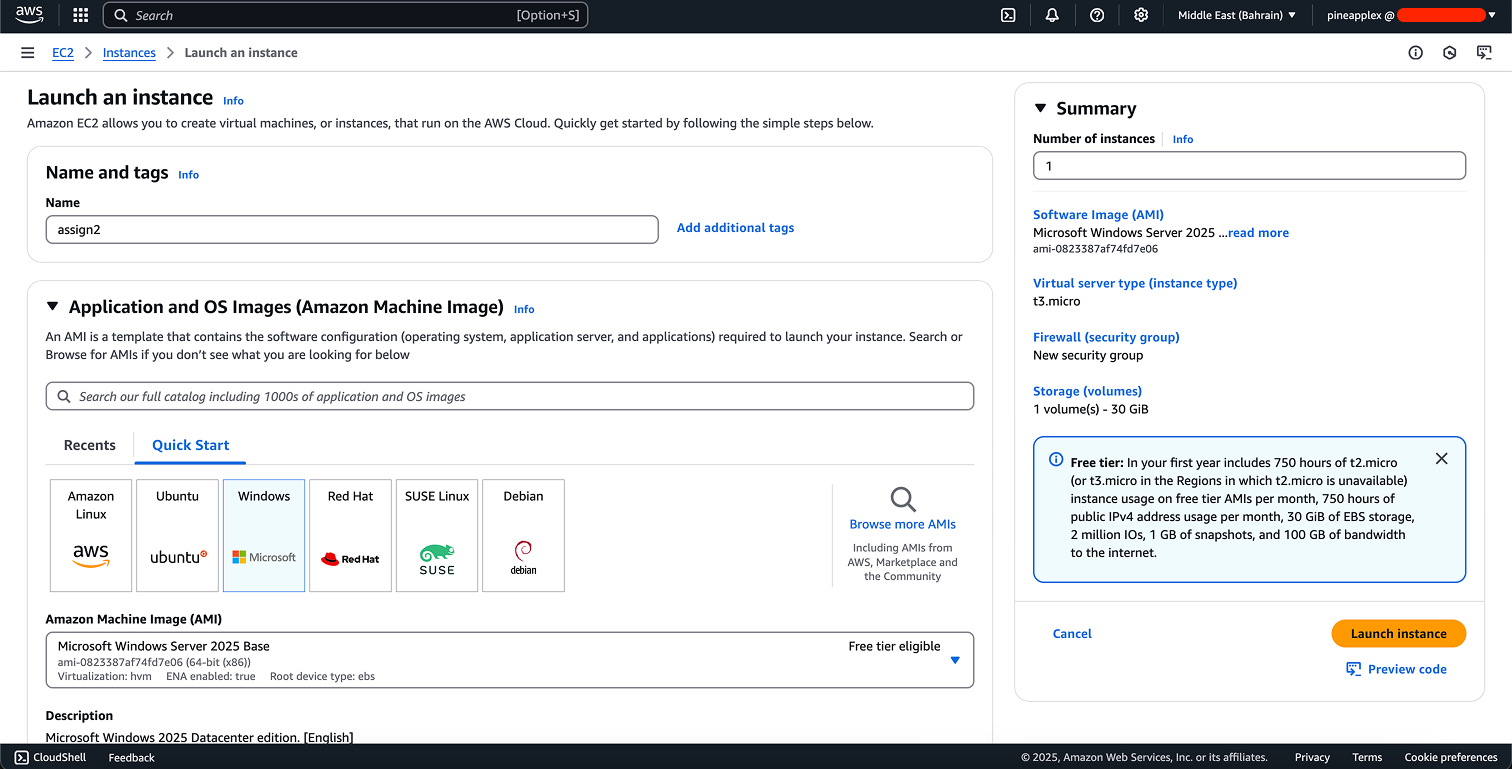
\includegraphics[width=0.95\textwidth]{create-windows-vm-1.png}
    \caption{Windows VM Creation - Initial Configuration with Windows Selected}
    \label{fig:windows-vm1}
\end{figure}

\begin{figure}[H]
    \centering
    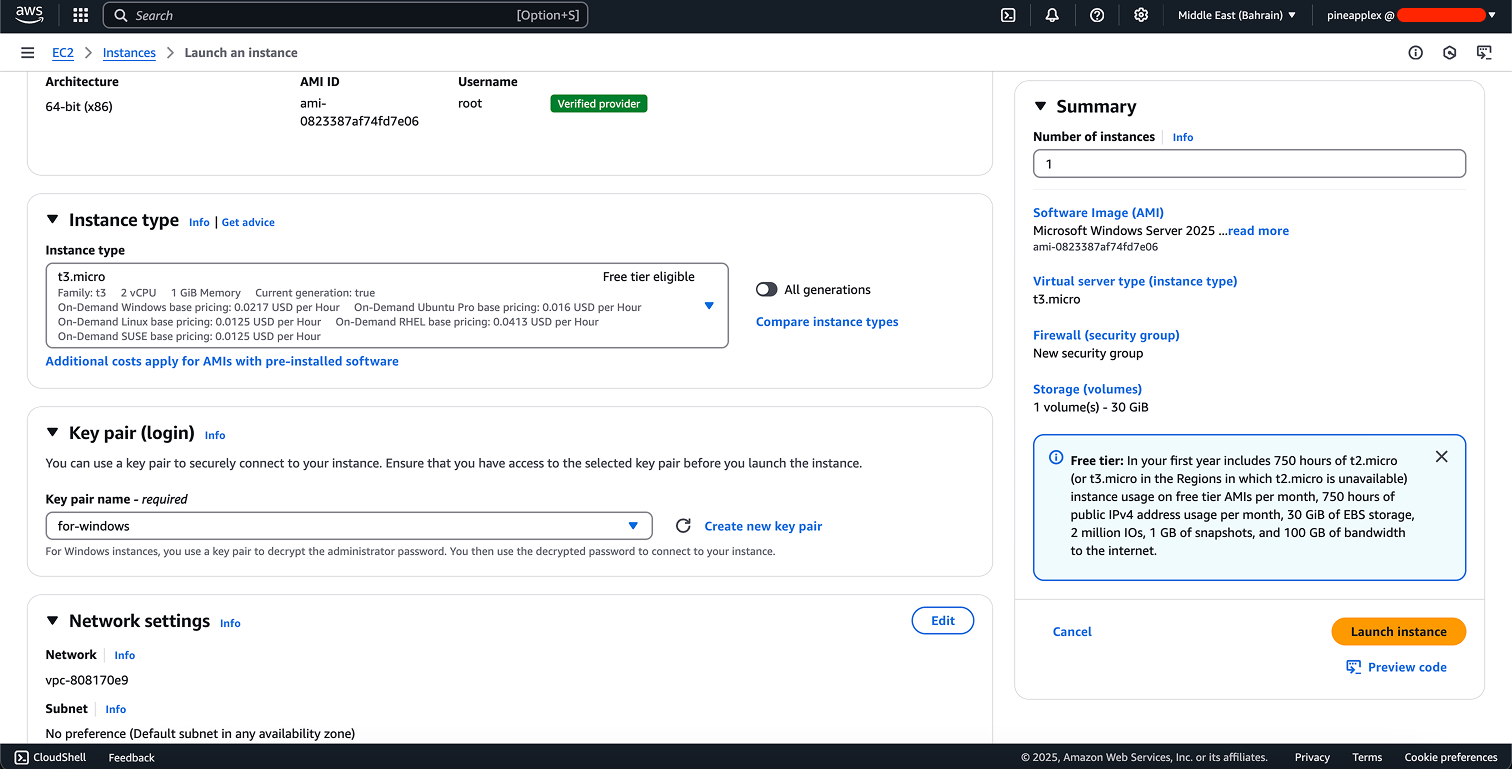
\includegraphics[width=0.95\textwidth]{create-windows-vm-2.png}
    \caption{Selecting t2.micro instance type for Windows Server and the New Key Pair}
    \label{fig:windows-vm2}
\end{figure}

\begin{figure}[H]
    \centering
    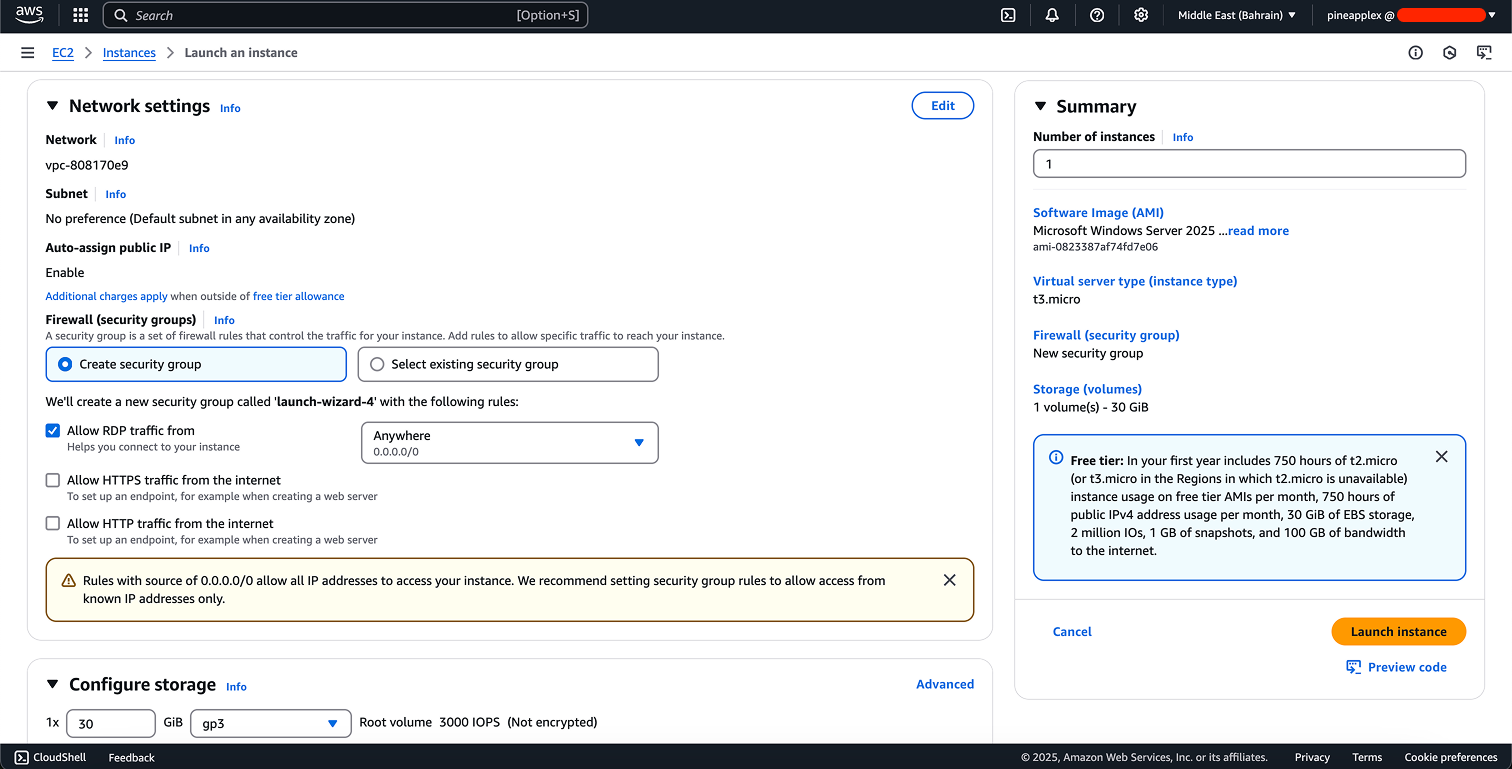
\includegraphics[width=0.95\textwidth]{create-windows-vm-3.png}
    \caption{Configuring VPC, subnet and security group settings}
    \label{fig:windows-vm3}
\end{figure}

\begin{figure}[H]
    \centering
    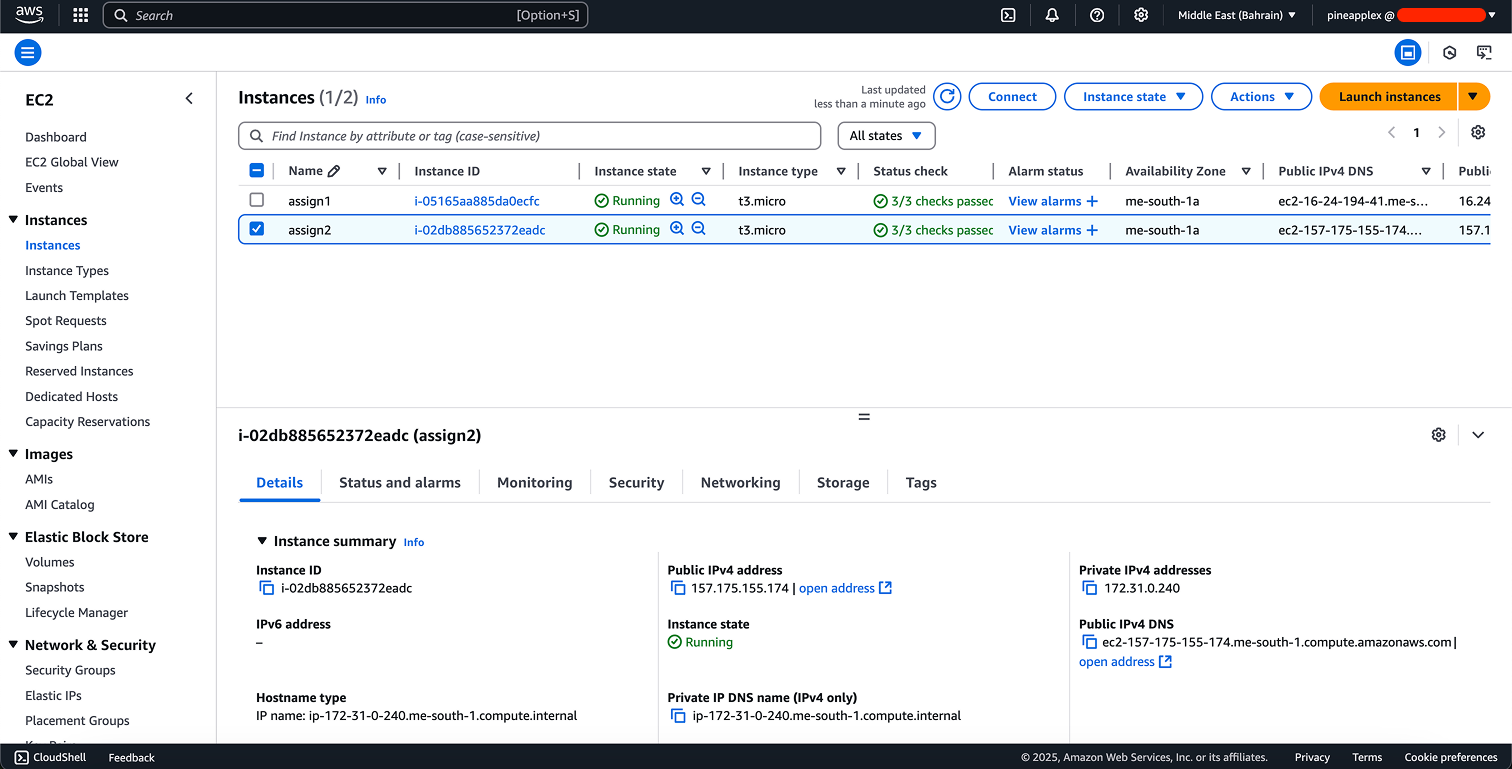
\includegraphics[width=0.95\textwidth]{create-windows-vm-4.png}
    \caption{Instance launch status confirmation page}
    \label{fig:windows-vm4}
\end{figure}

\subsection{Connect to VM}

\begin{figure}[H]
    \centering
    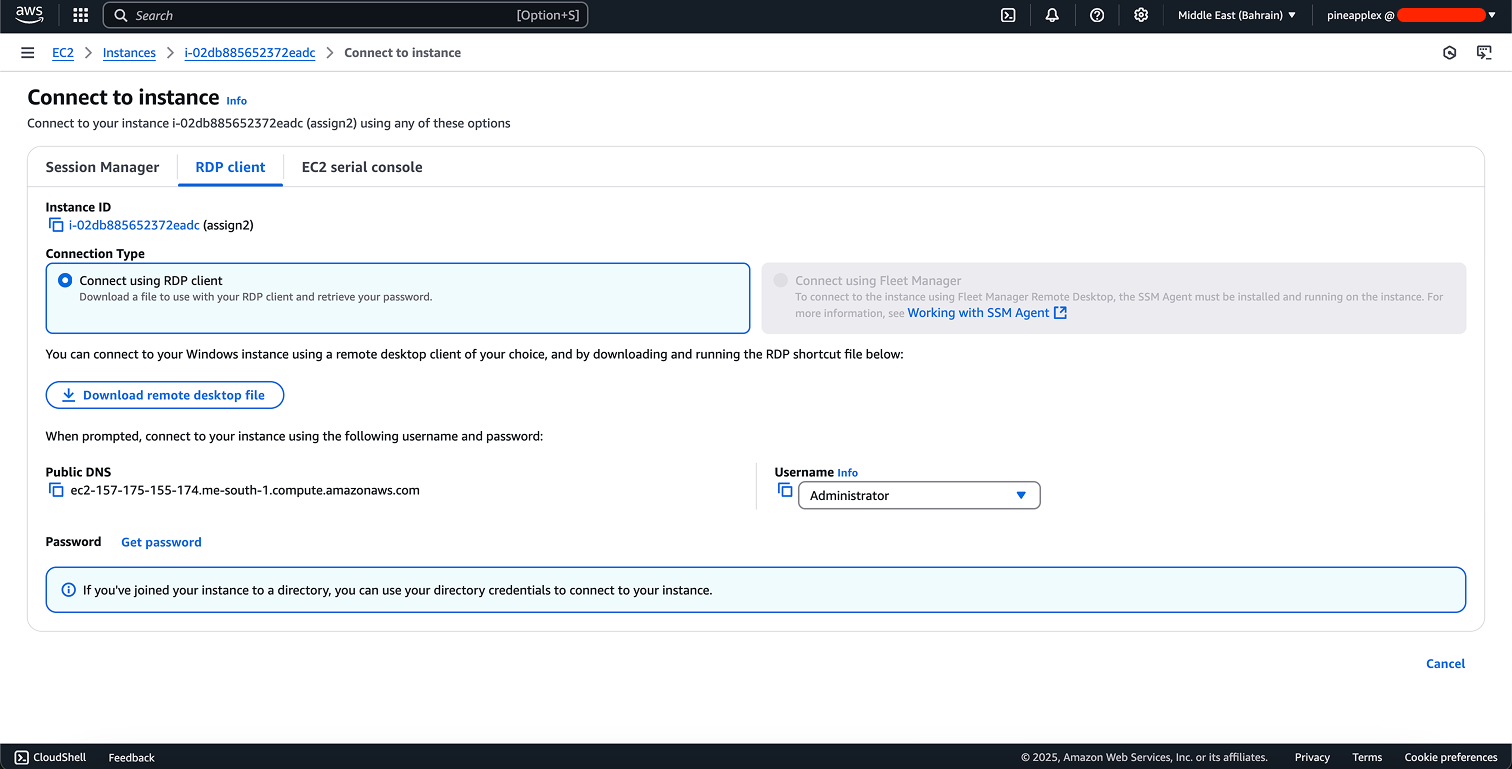
\includegraphics[width=0.95\textwidth]{connect-to-vm-1.png}
    \caption{Setup Connect Using RDP Client}
    \label{fig:connect1}
\end{figure}

\begin{figure}[H]
    \centering
    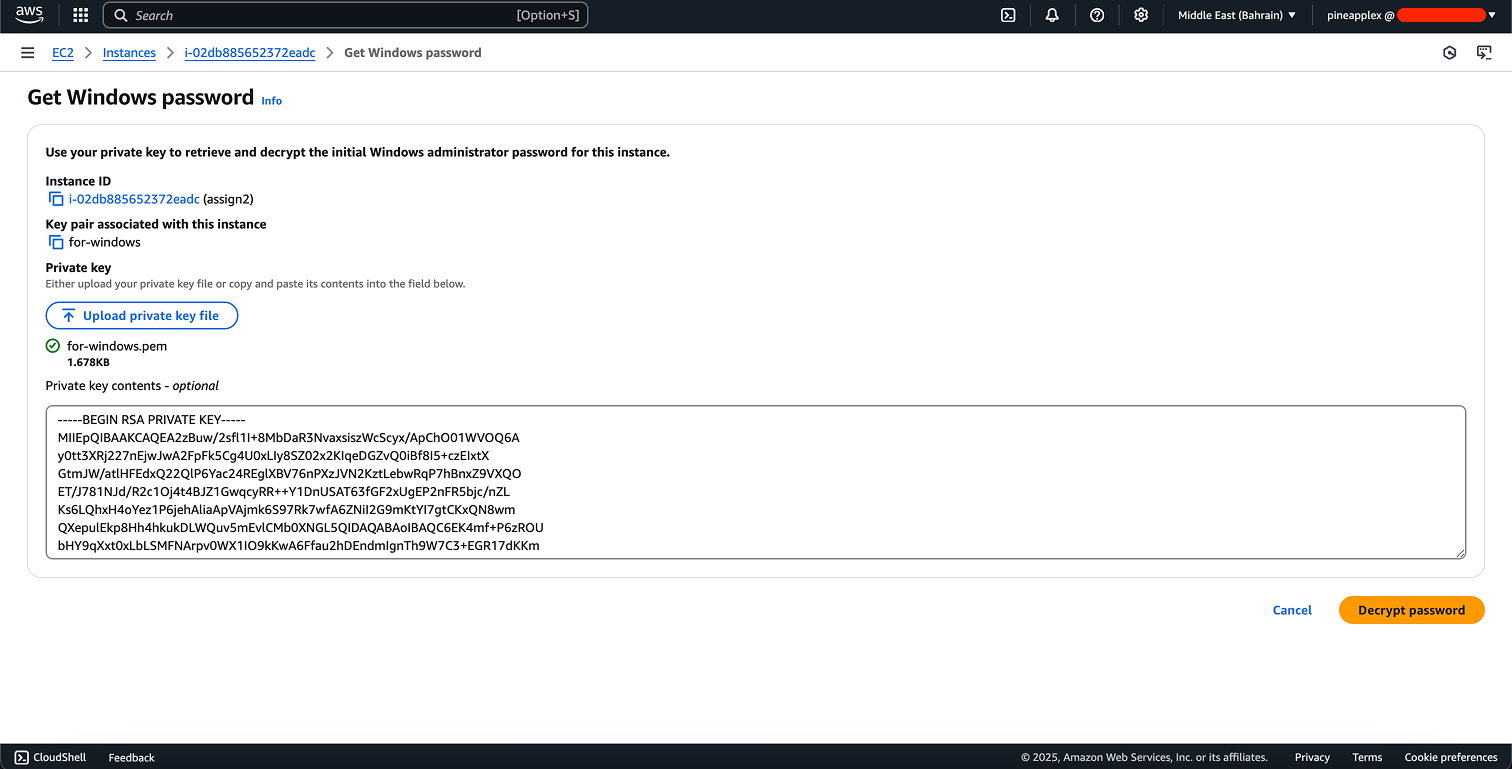
\includegraphics[width=0.95\textwidth]{connect-to-vm-2.png}
    \caption{Uploading Private Key to Decrypt Windows Password}
    \label{fig:connect2}
\end{figure}

\begin{figure}[H]
    \centering
    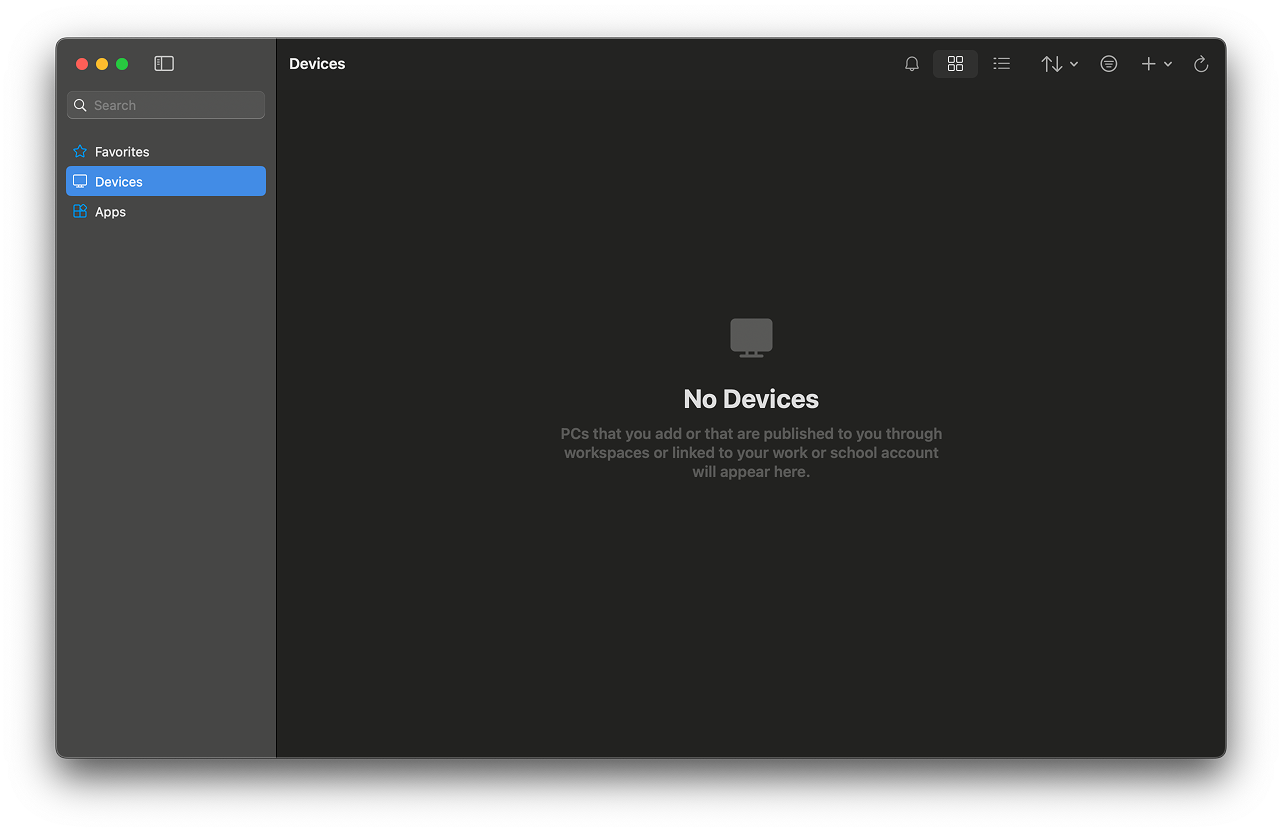
\includegraphics[width=0.95\textwidth]{connect-to-vm-3.png}
    \caption{Opened RDP Client for Windows "Windows App Beta" on macOS}
    \label{fig:connect3}
\end{figure}

\begin{figure}[H]
    \centering
    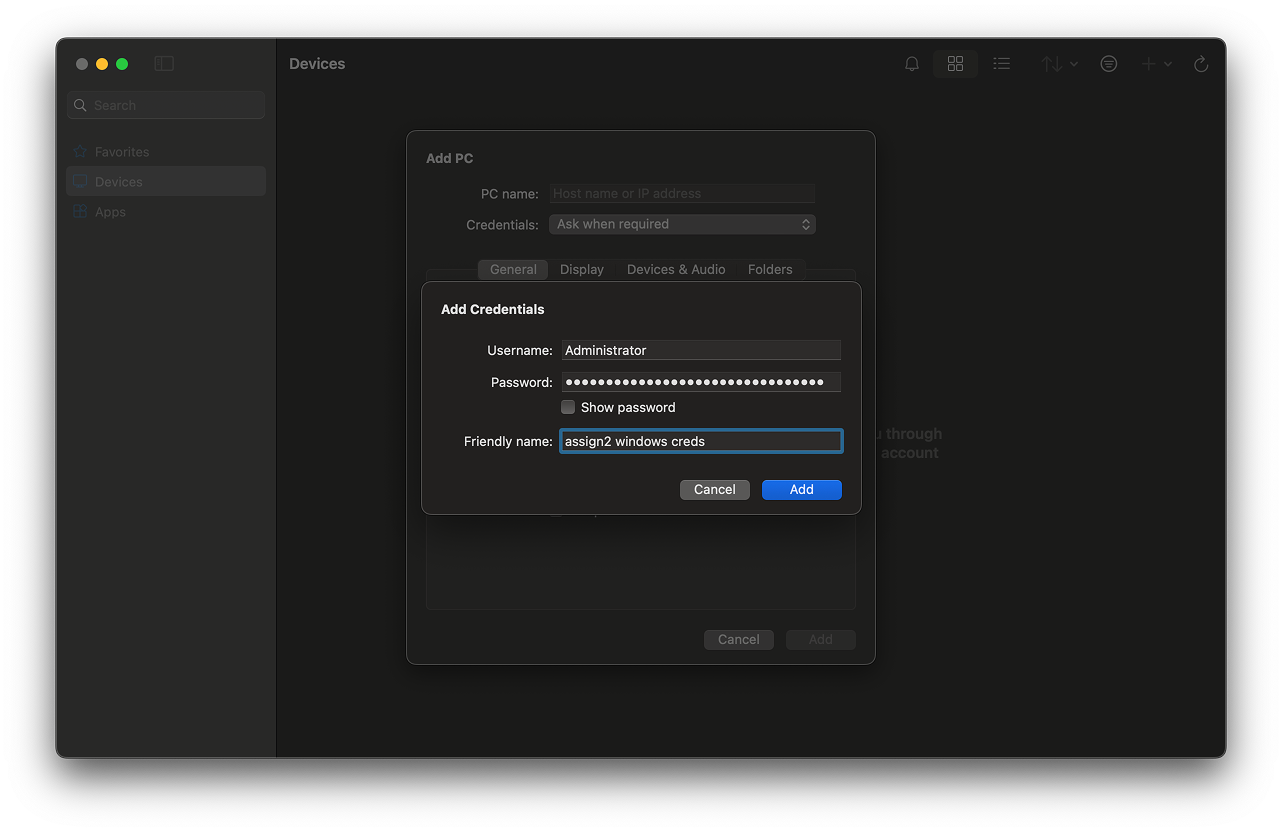
\includegraphics[width=0.95\textwidth]{connect-to-vm-4.png}
    \caption{Add Credentials in RDP Client}
    \label{fig:connect4}
\end{figure}

\begin{figure}[H]
    \centering
    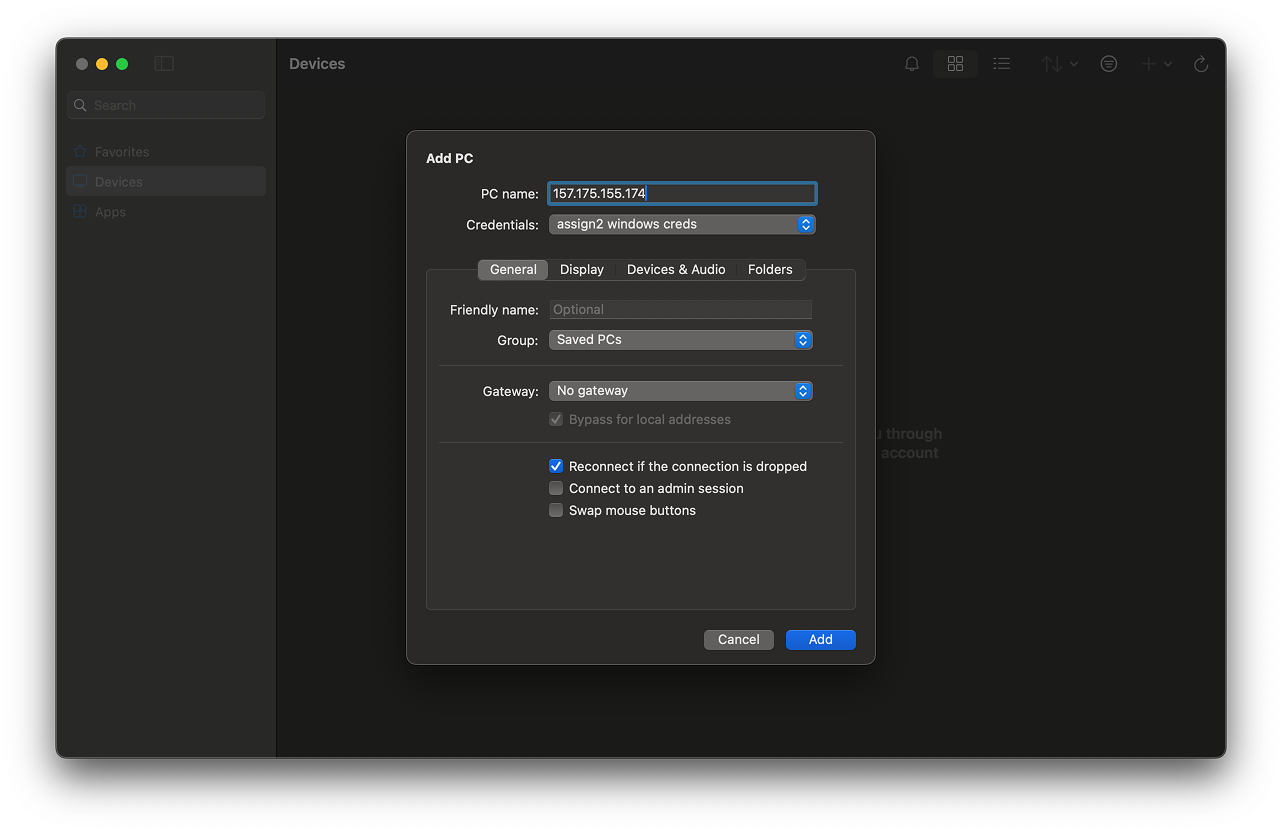
\includegraphics[width=0.95\textwidth]{connect-to-vm-5.png}
    \caption{Enter IP Address}
    \label{fig:connect5}
\end{figure}

\begin{figure}[H]
    \centering
    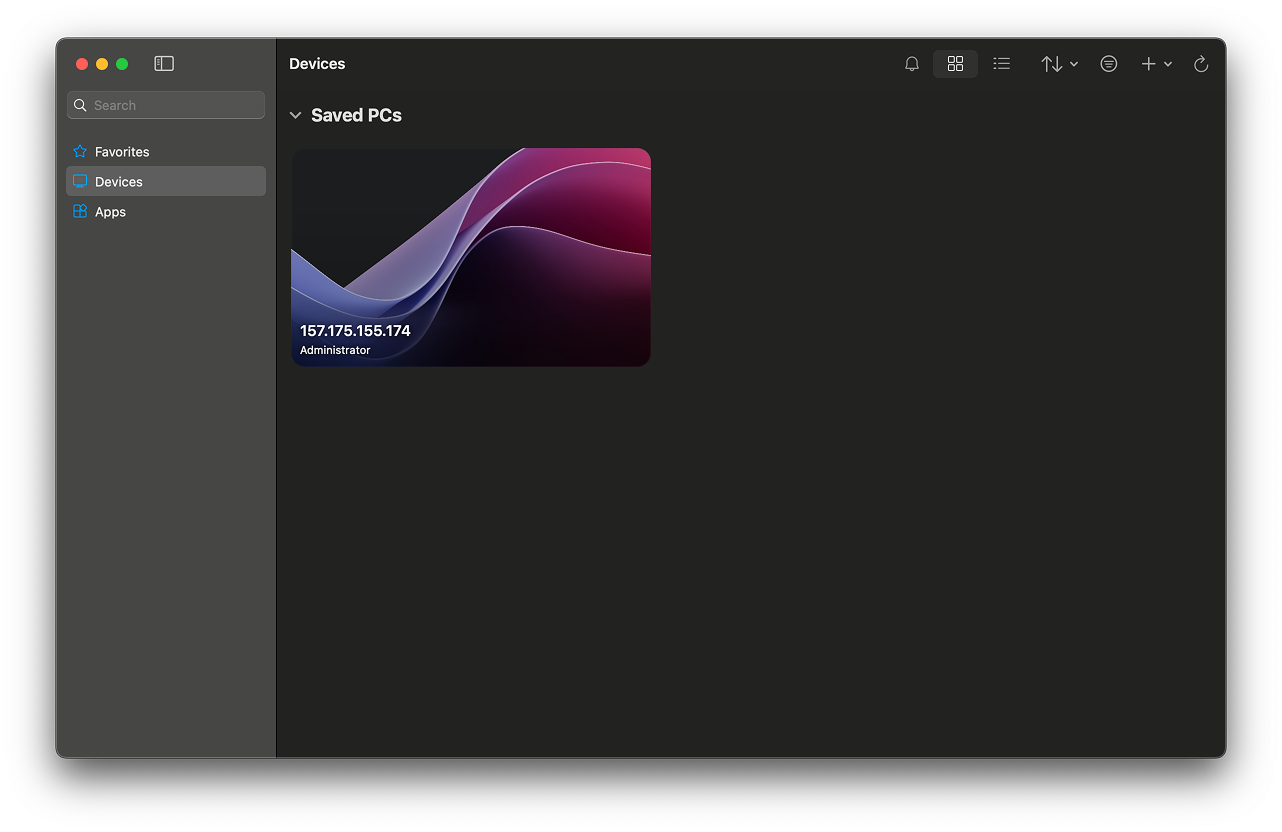
\includegraphics[width=0.95\textwidth]{connect-to-vm-6.png}
    \caption{PC Added Successfully}
    \label{fig:connect6}
\end{figure}

\begin{figure}[H]
    \centering
    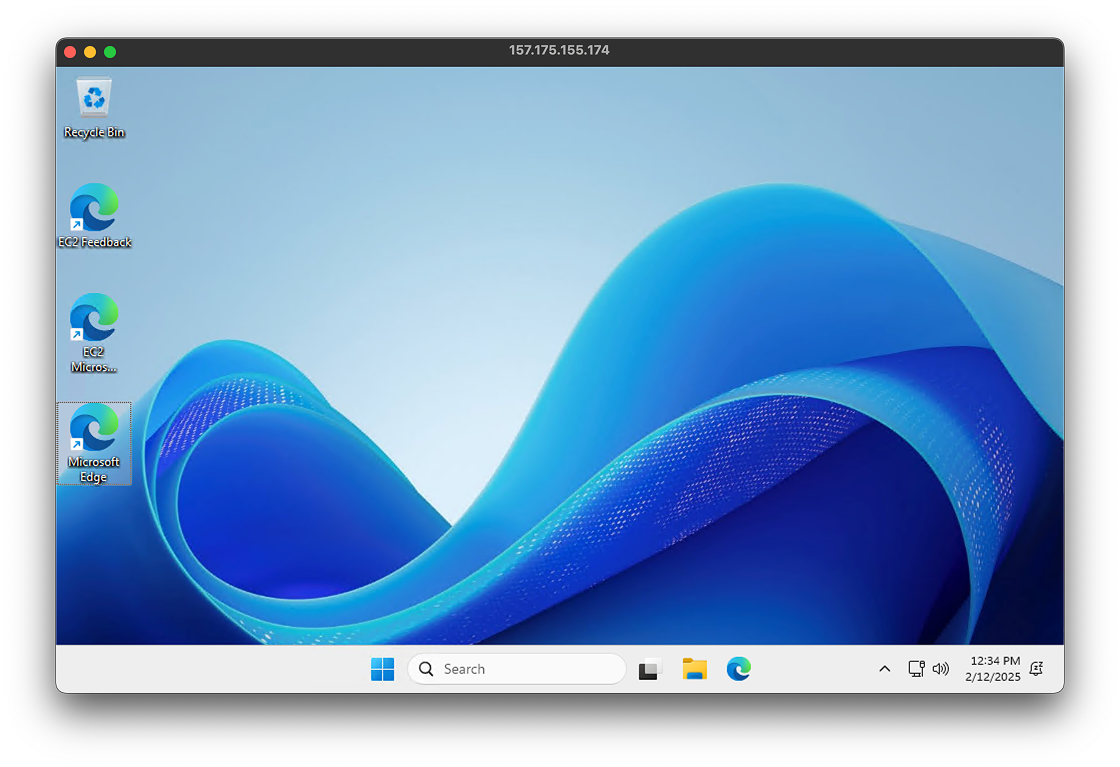
\includegraphics[width=0.95\textwidth]{connect-to-vm-7.png}
    \caption{Successfully Connected}
    \label{fig:connect7}
\end{figure}

\section{Part B: Create Snapshots / Backups/Amazon Machine Image (AMI) Creation}

\begin{figure}[H]
    \centering
    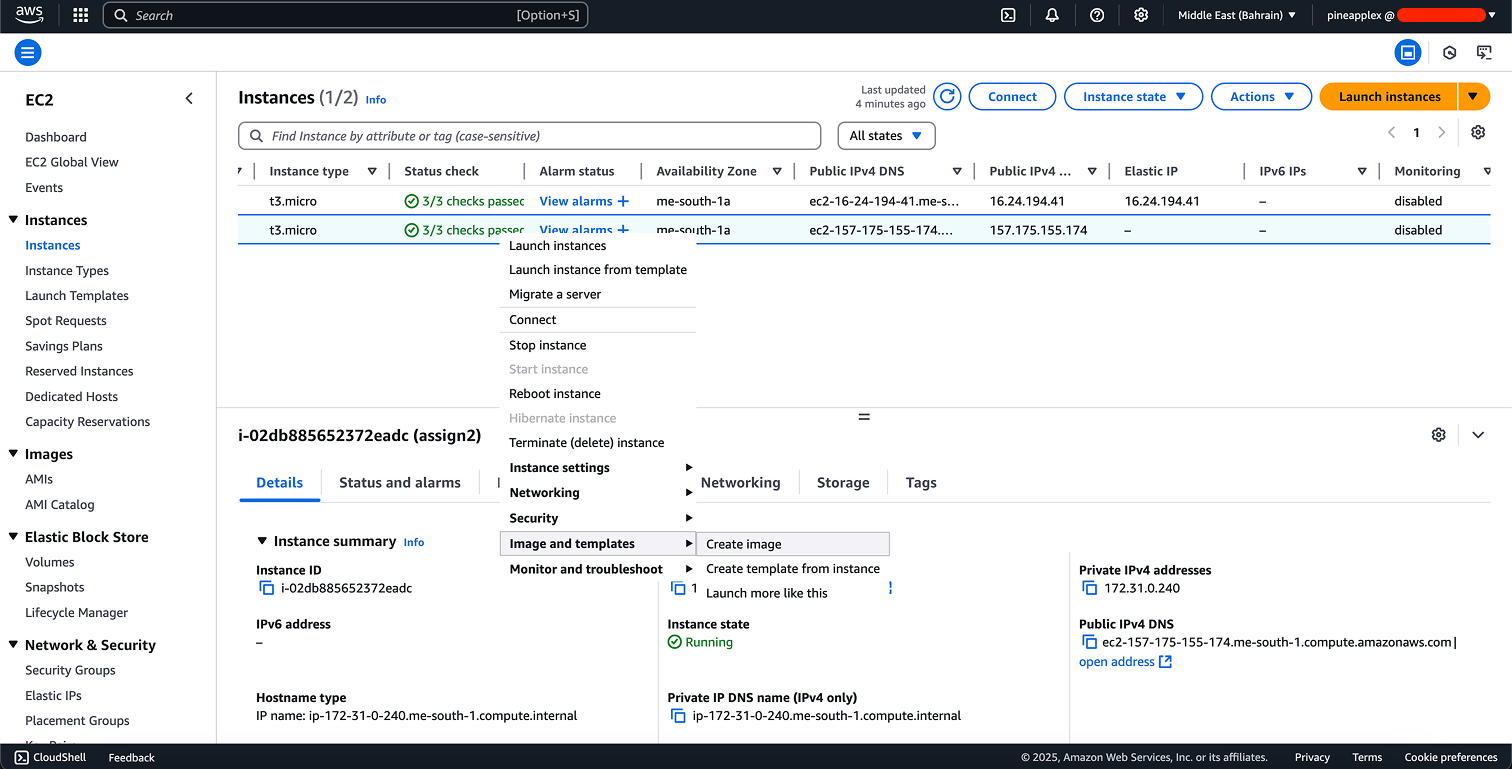
\includegraphics[width=0.95\textwidth]{create-image-1.png}
    \caption{Right Click to Create Image}
    \label{fig:image1}
\end{figure}

\begin{figure}[H]
    \centering
    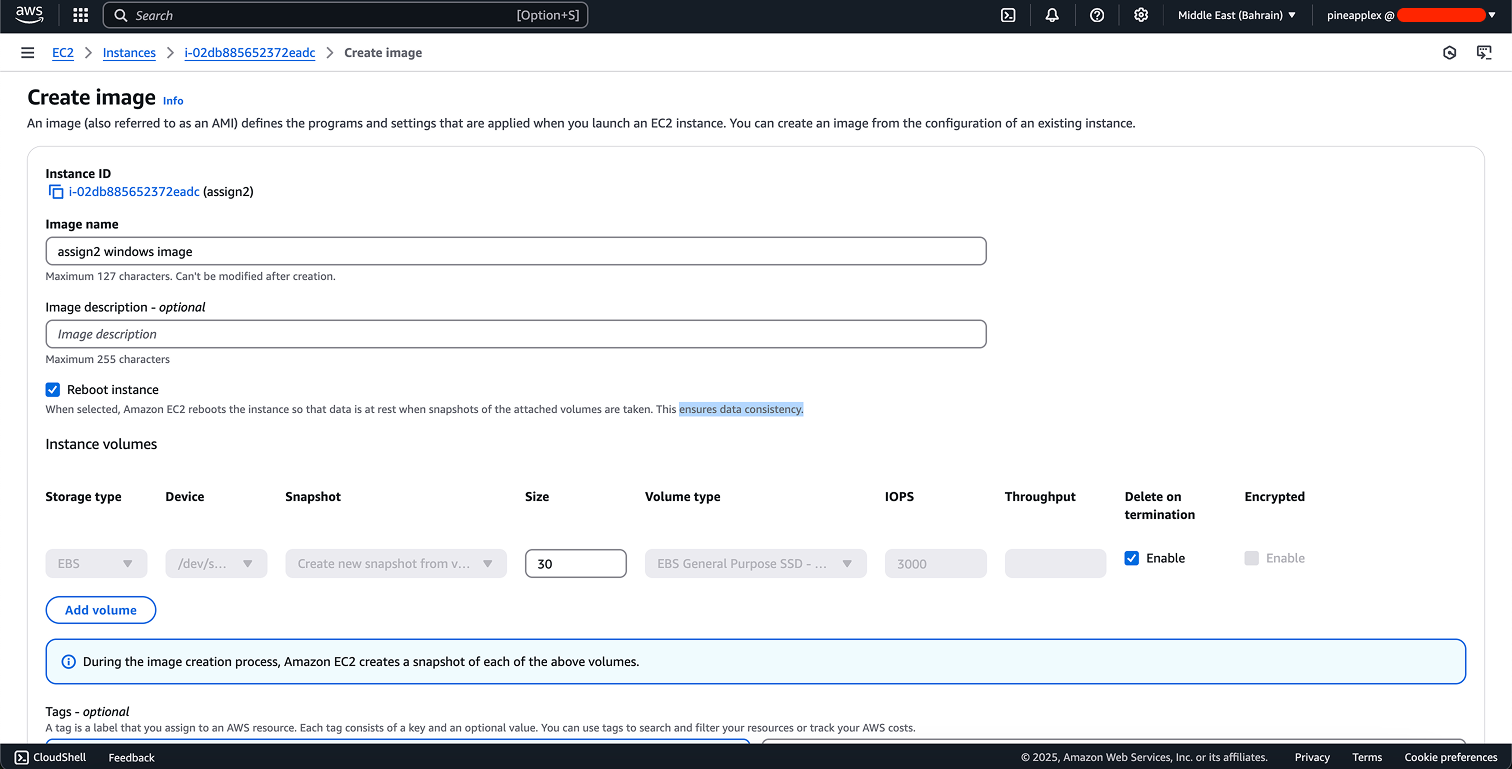
\includegraphics[width=0.95\textwidth]{create-image-2.png}
    \caption{AMI Creation Options}
    \label{fig:image2}
\end{figure}

\begin{figure}[H]
    \centering
    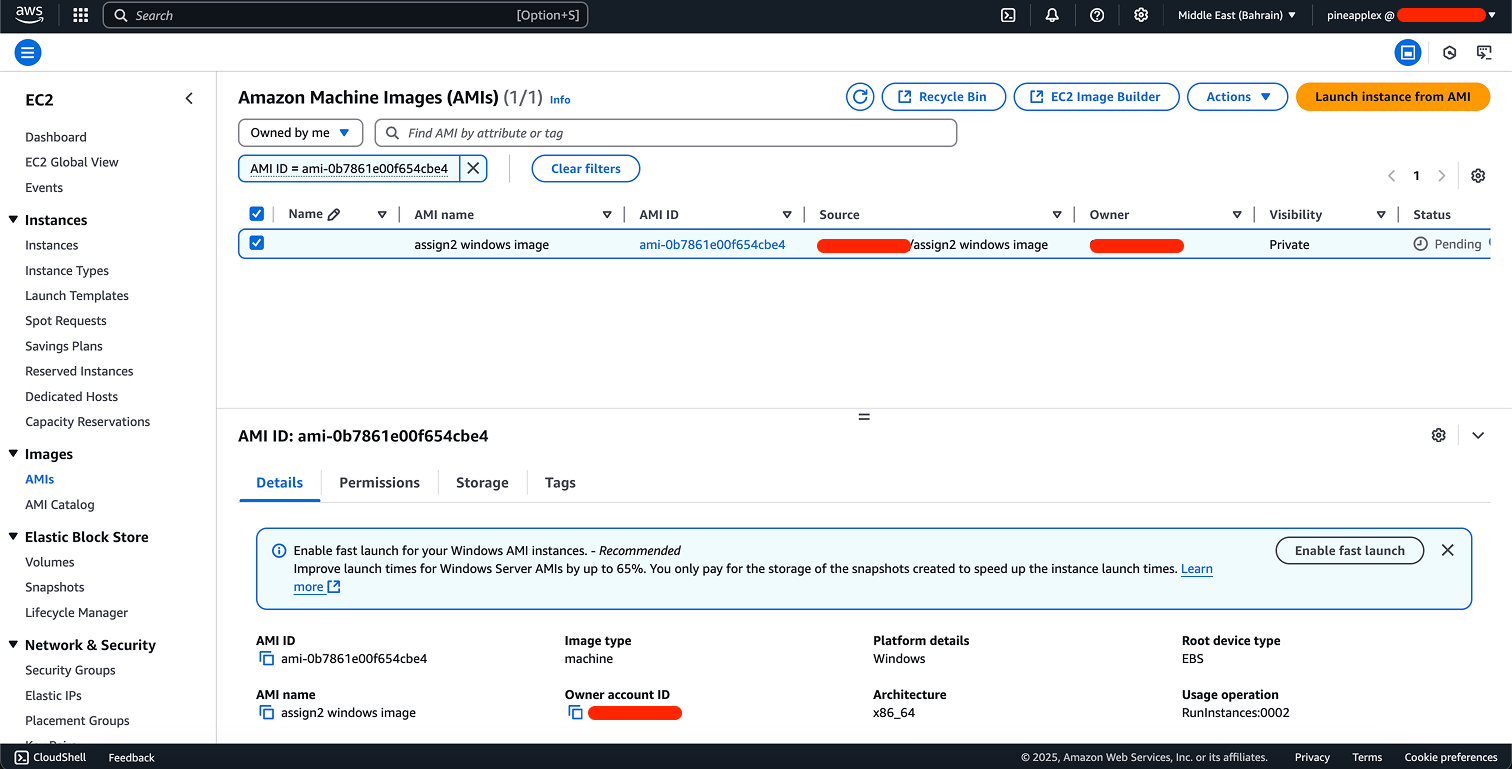
\includegraphics[width=0.95\textwidth]{create-image-3.png}
    \caption{AMI Created Successfully}
    \label{fig:image3}
\end{figure}

\section{Part C: How to host a static website on AWS S3}

\begin{figure}[H]
    \centering
    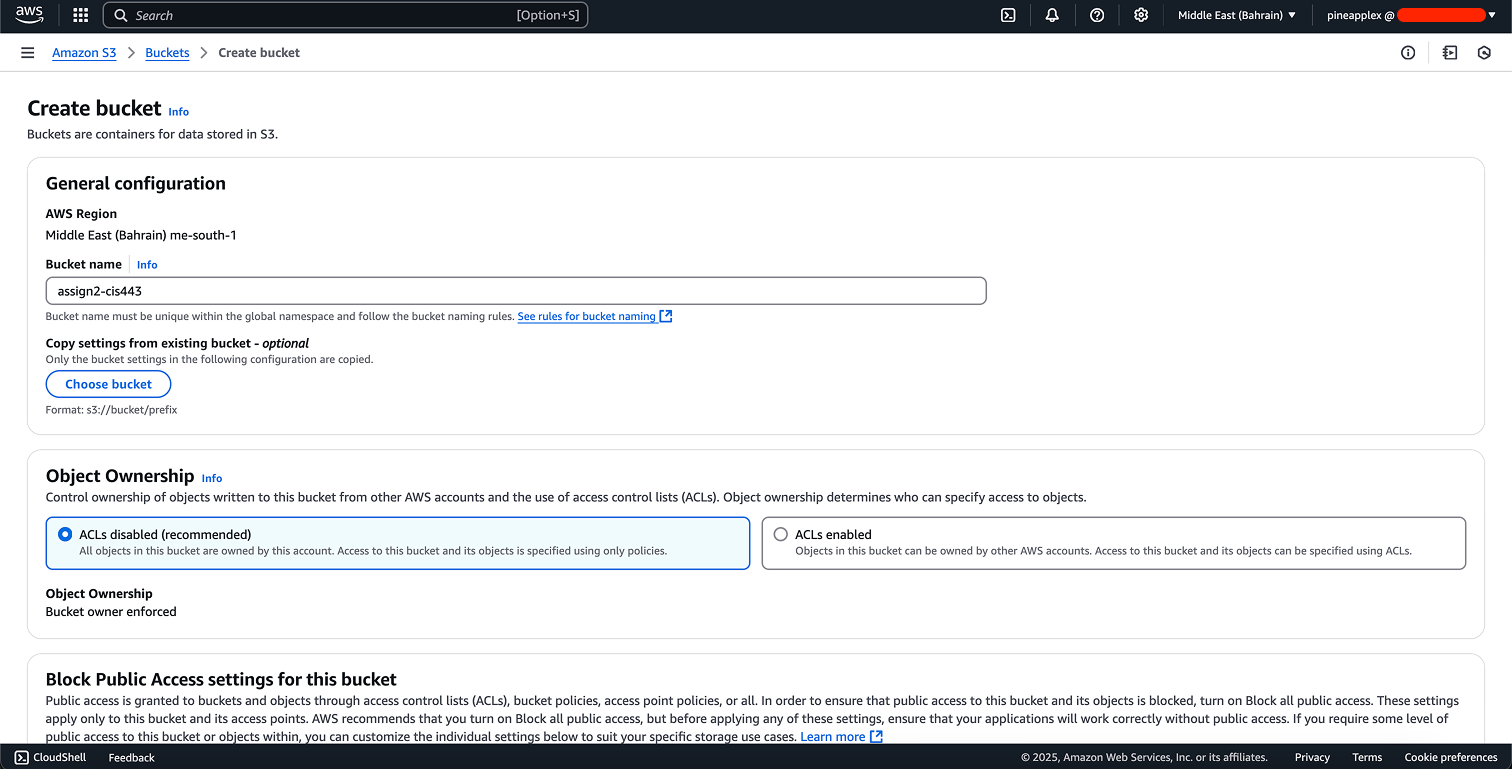
\includegraphics[width=0.95\textwidth]{host-static-website-1.png}
    \caption{Bucket Creation 1}
    \label{fig:static1}
\end{figure}

\begin{figure}[H]
    \centering
    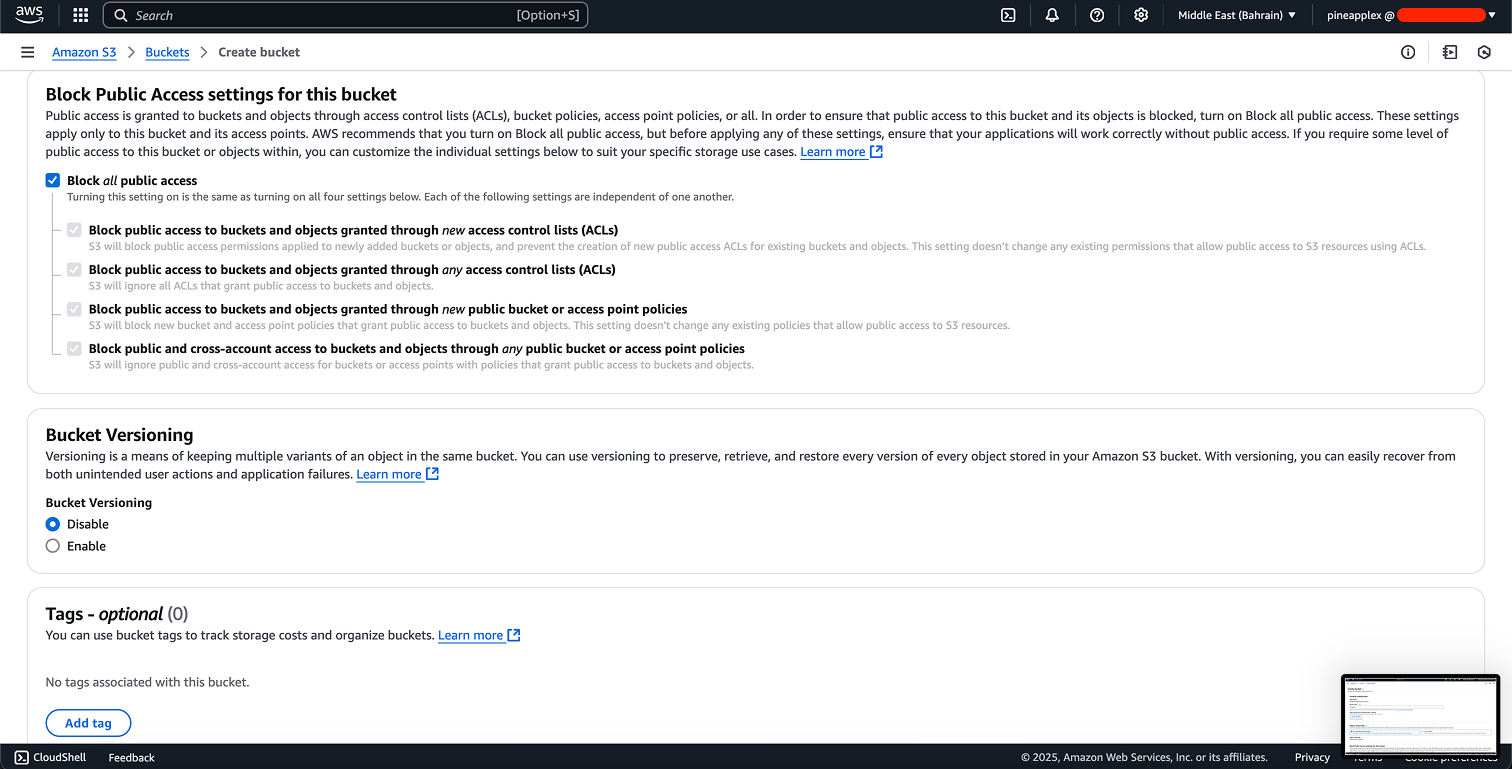
\includegraphics[width=0.95\textwidth]{host-static-website-2.png}
    \caption{Bucket Creation 2}
    \label{fig:static2}
\end{figure}

\begin{figure}[H]
    \centering
    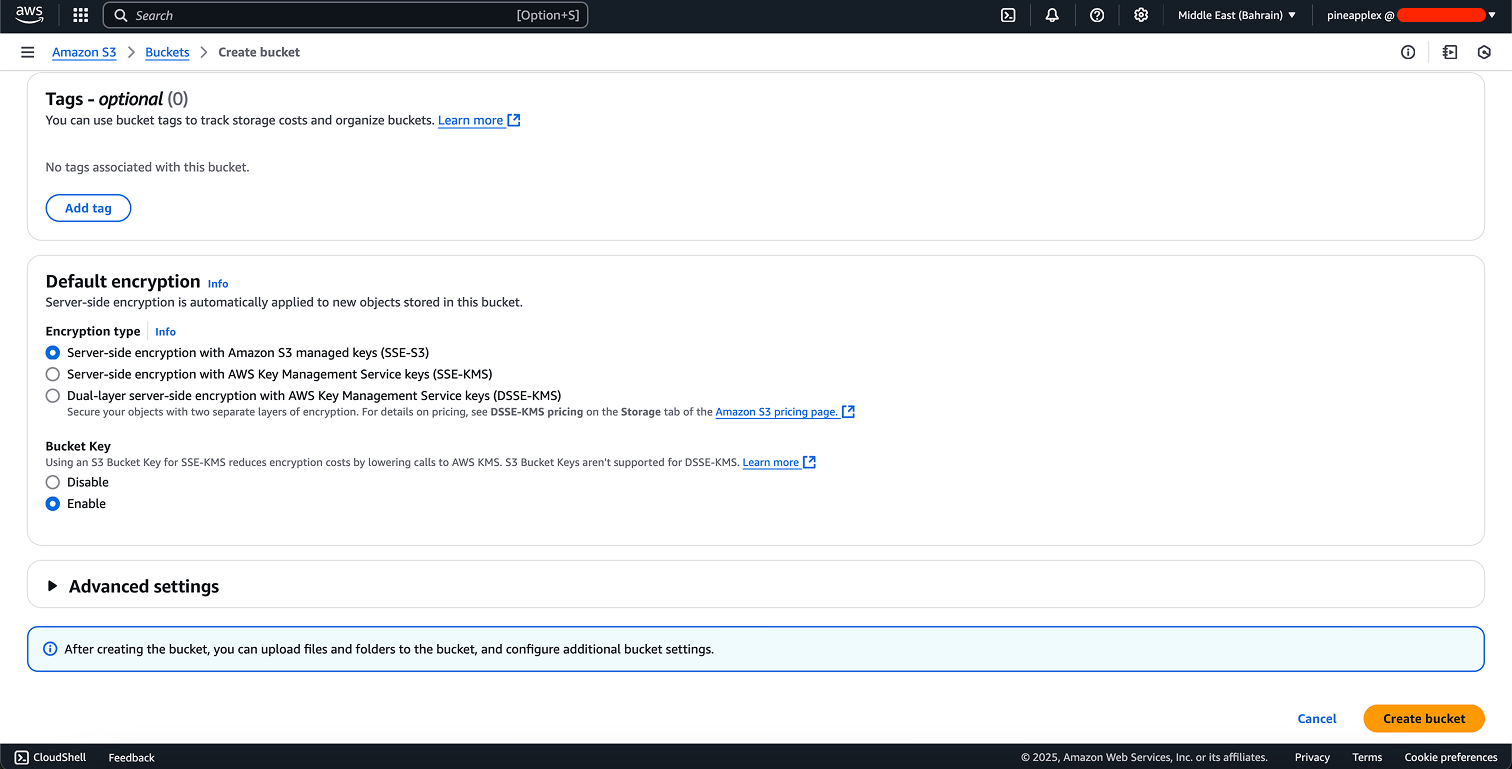
\includegraphics[width=0.95\textwidth]{host-static-website-3.png}
    \caption{Bucket Creation 3}
    \label{fig:static3}
\end{figure}

\begin{figure}[H]
    \centering
    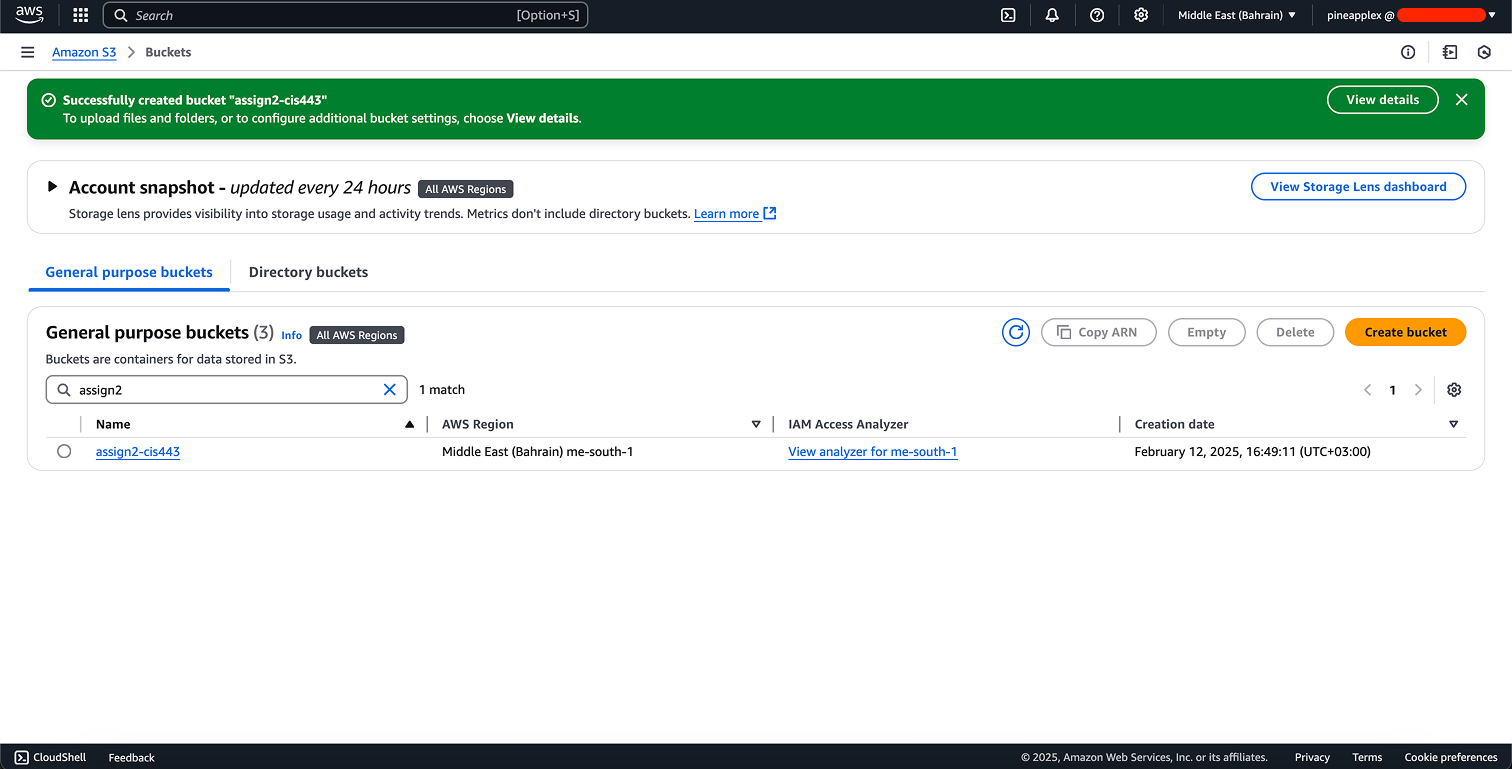
\includegraphics[width=0.95\textwidth]{host-static-website-4.png}
    \caption{Created Bucket Successfully}
    \label{fig:static4}
\end{figure}

\begin{figure}[H]
    \centering
    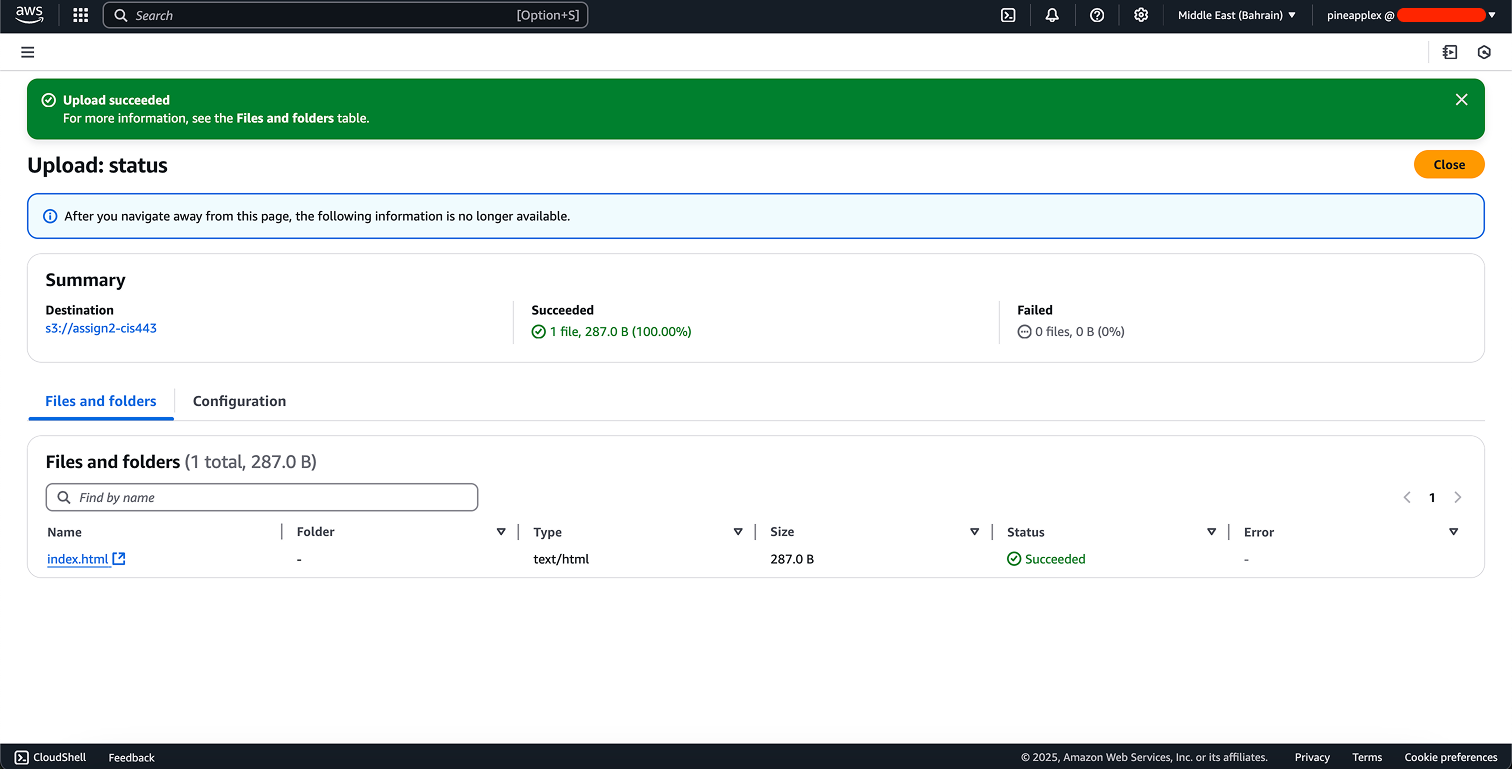
\includegraphics[width=0.95\textwidth]{host-static-website-5.png}
    \caption{Uploaded \texttt{index.html} File Successfully}
    \label{fig:static5}
\end{figure}

\begin{figure}[H]
    \centering
    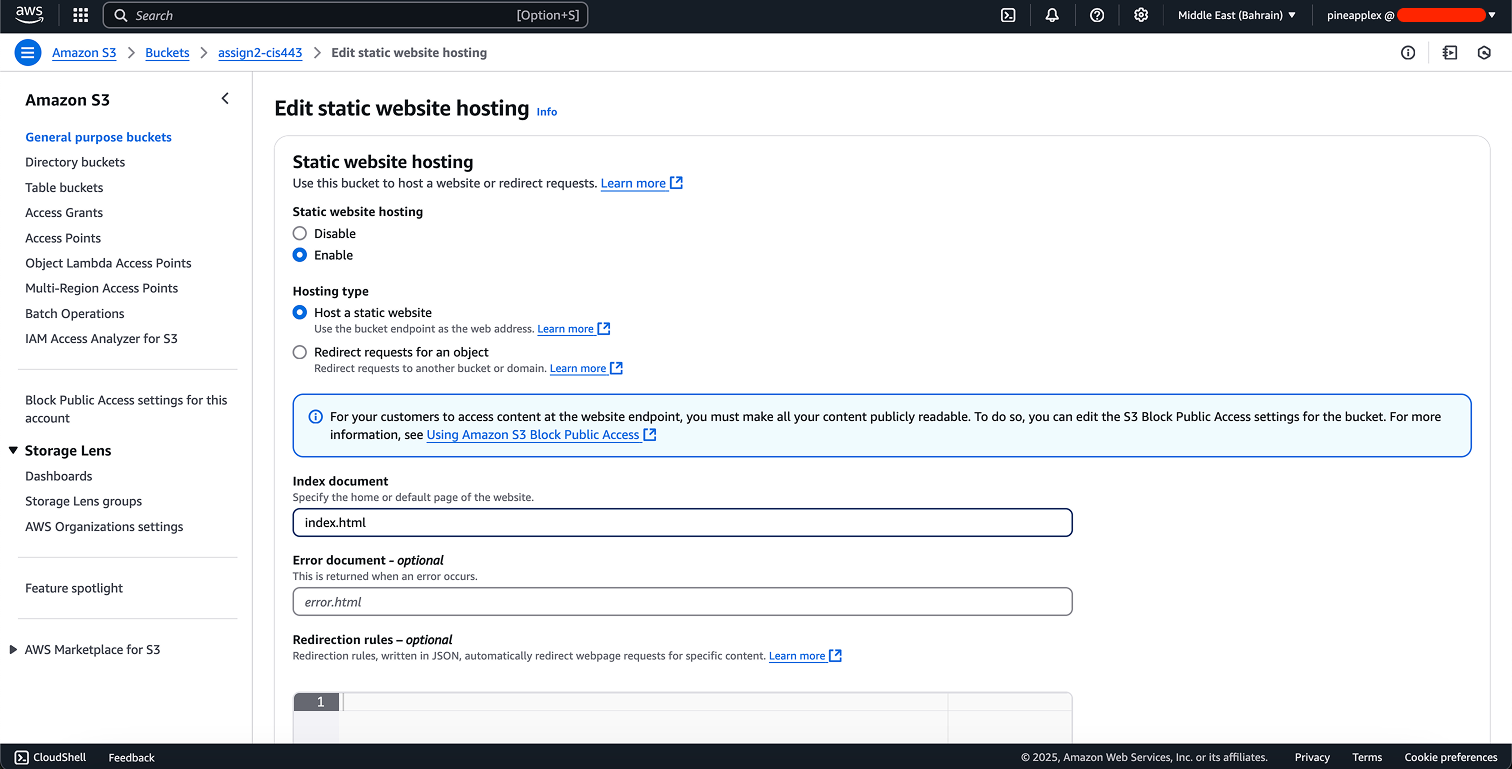
\includegraphics[width=0.95\textwidth]{host-static-website-6.png}
    \caption{Static Web Hosting Setting Page}
    \label{fig:static6}
\end{figure}

\begin{figure}[H]
    \centering
    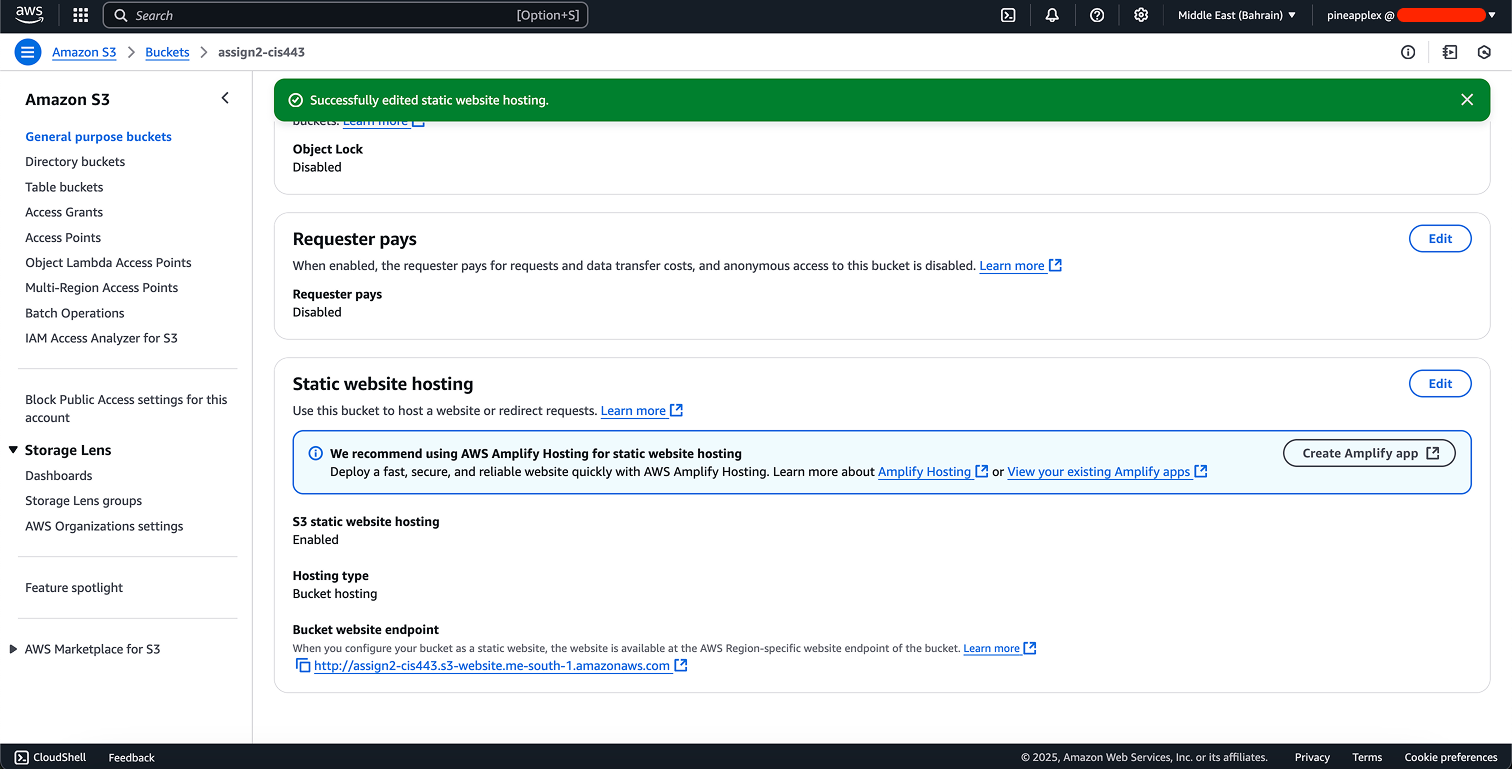
\includegraphics[width=0.95\textwidth]{host-static-website-7.png}
    \caption{Static Website Hosting Enabled}
    \label{fig:static7}
\end{figure}

\begin{figure}[H]
    \centering
    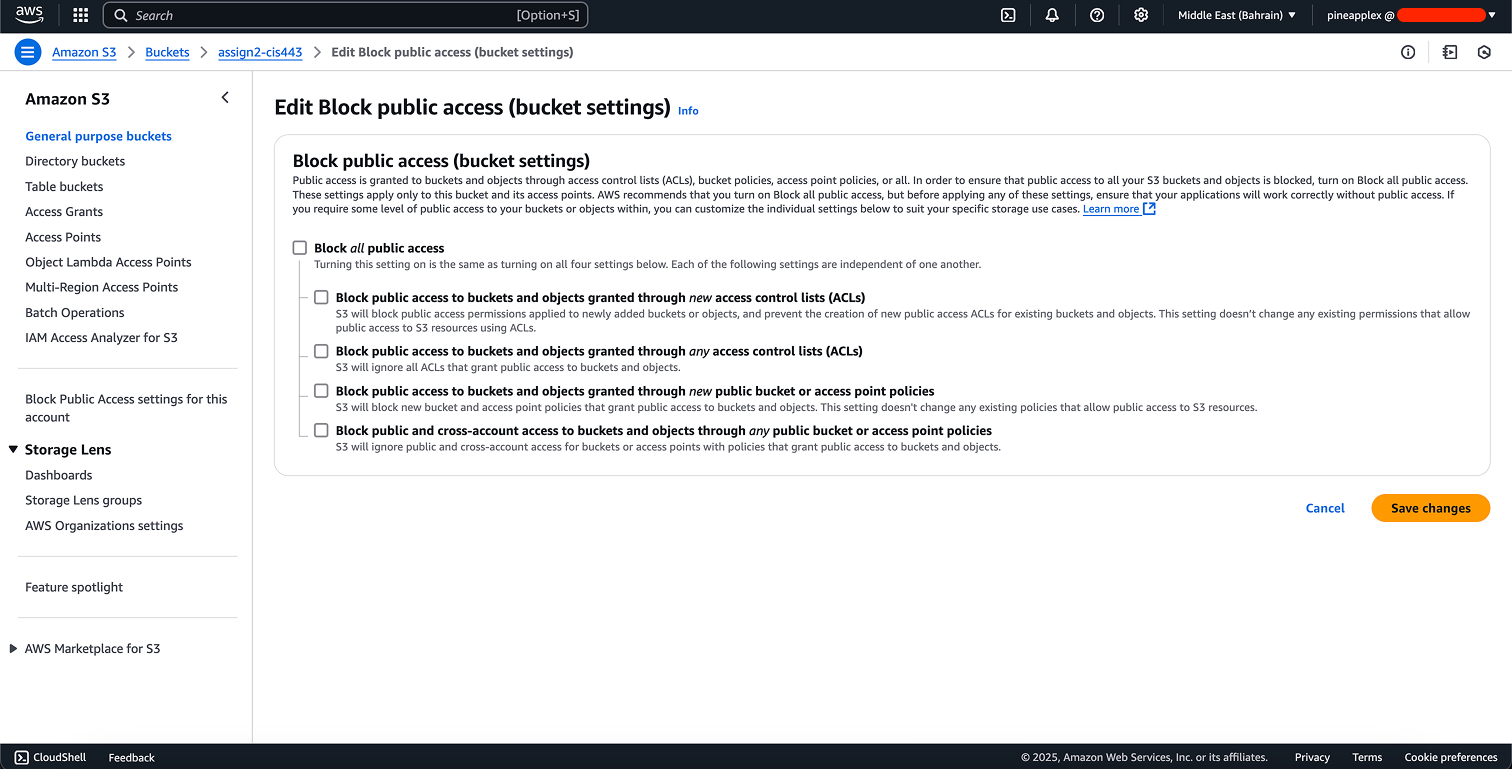
\includegraphics[width=0.95\textwidth]{host-static-website-8.png}
    \caption{Disabled "Block Public Access" Setting}
    \label{fig:static8}
\end{figure}

\begin{figure}[H]
    \centering
    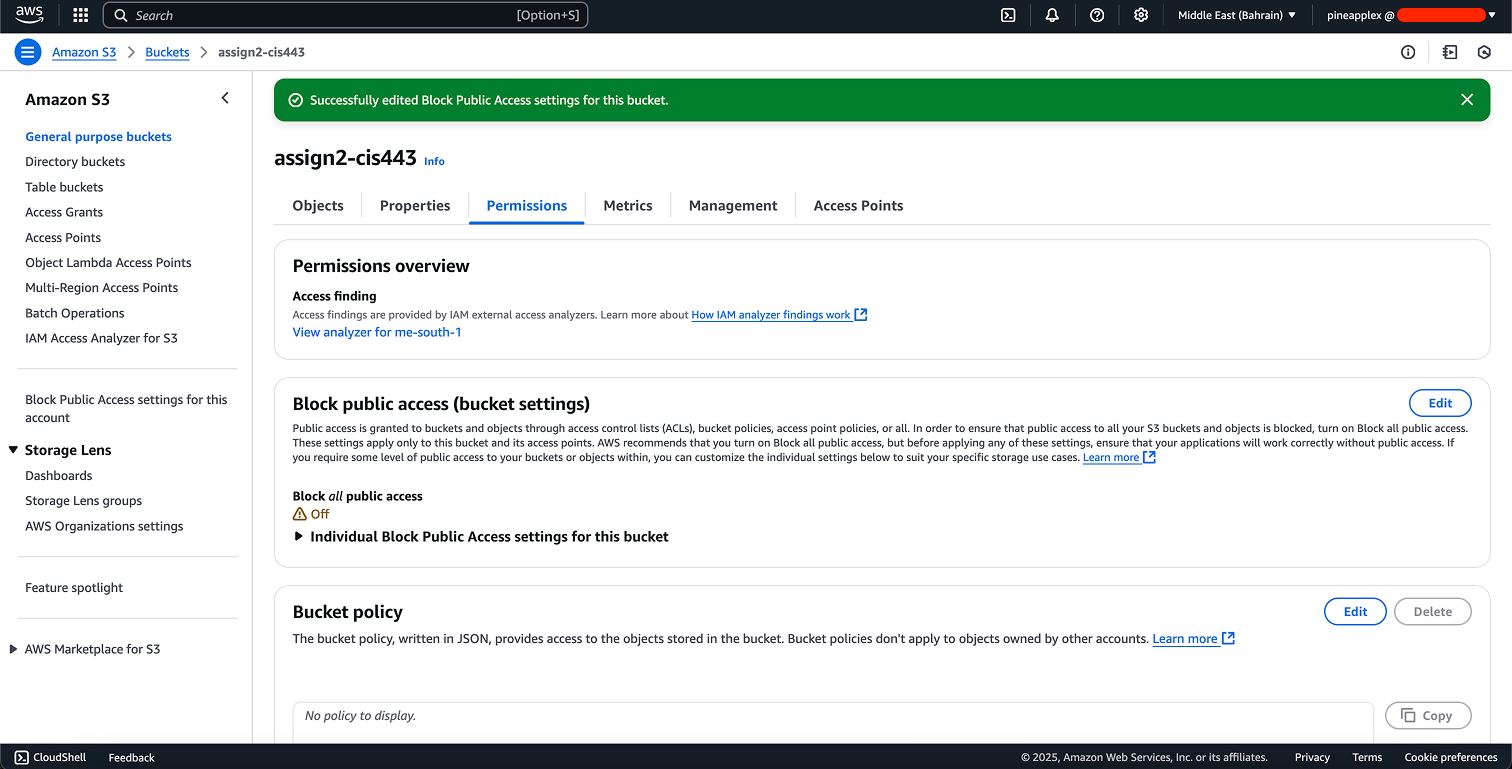
\includegraphics[width=0.95\textwidth]{host-static-website-9.png}
    \caption{Success Page for "Block Public Access" Being Disabled}
    \label{fig:static9}
\end{figure}

\begin{figure}[H]
    \centering
    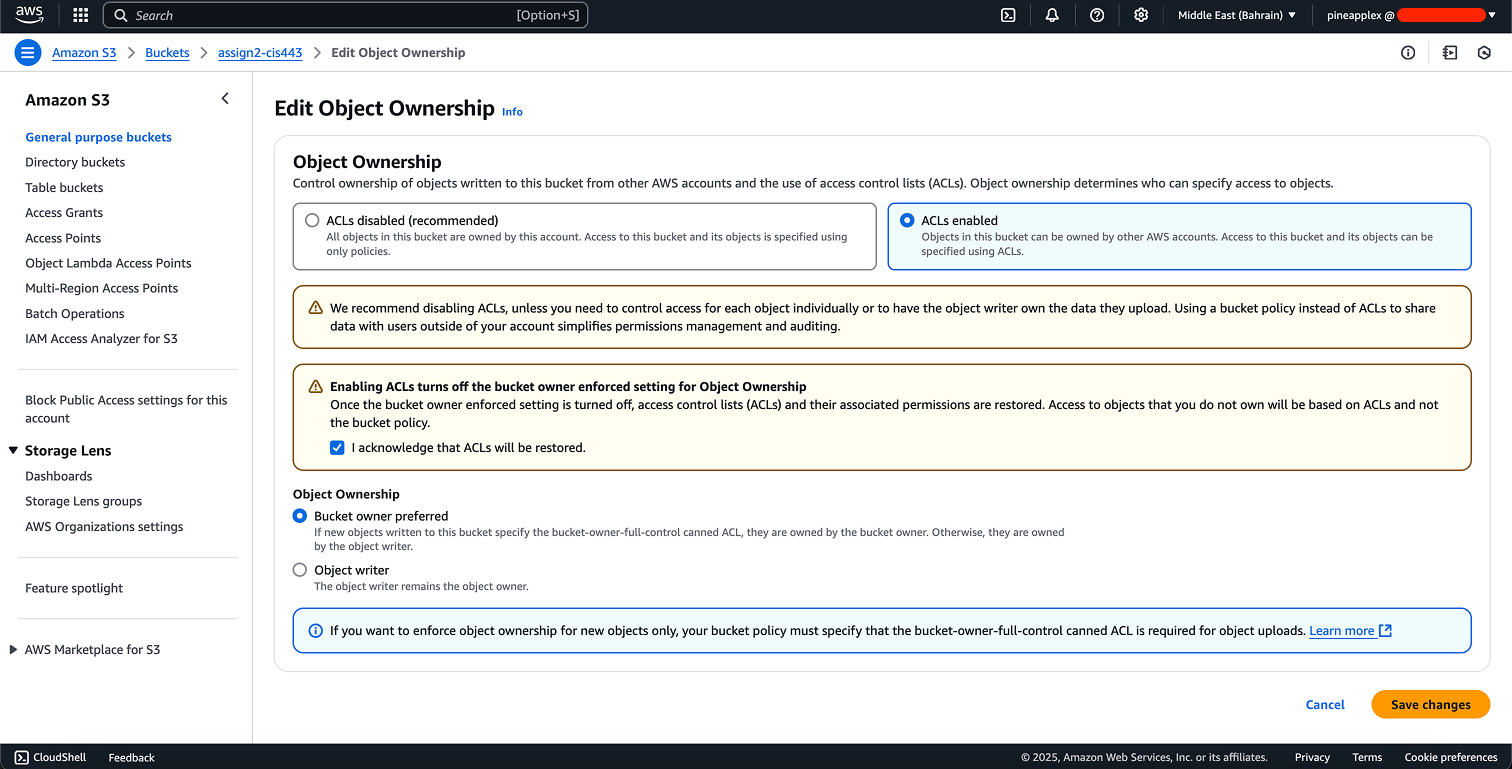
\includegraphics[width=0.95\textwidth]{host-static-website-10.png}
    \caption{Object Ownership Setting Change to Enable ACL}
    \label{fig:static10}
\end{figure}

\begin{figure}[H]
    \centering
    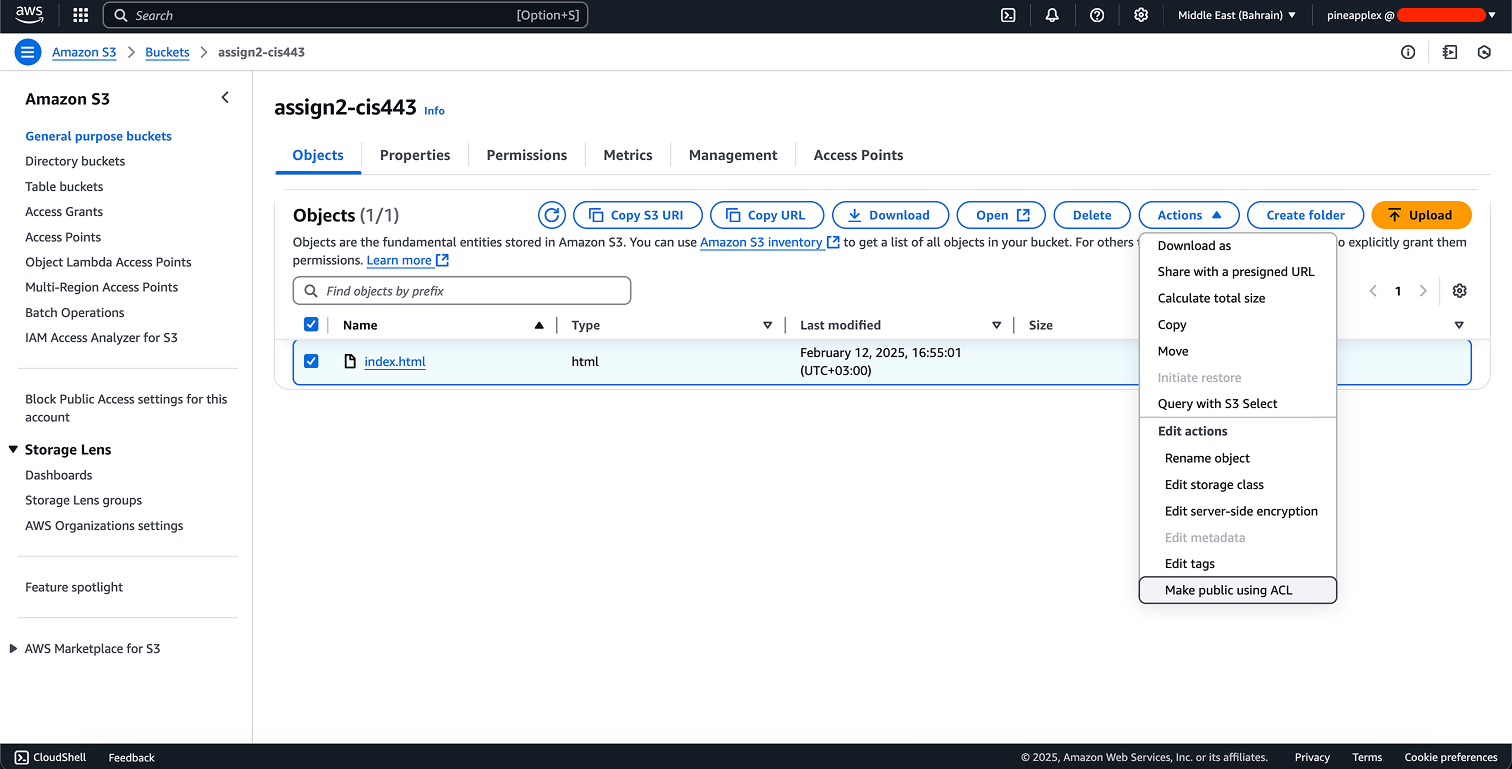
\includegraphics[width=0.95\textwidth]{host-static-website-11.png}
    \caption{S3 Static Website - Make Public Menu Item}
    \label{fig:static11}
\end{figure}

\begin{figure}[H]
    \centering
    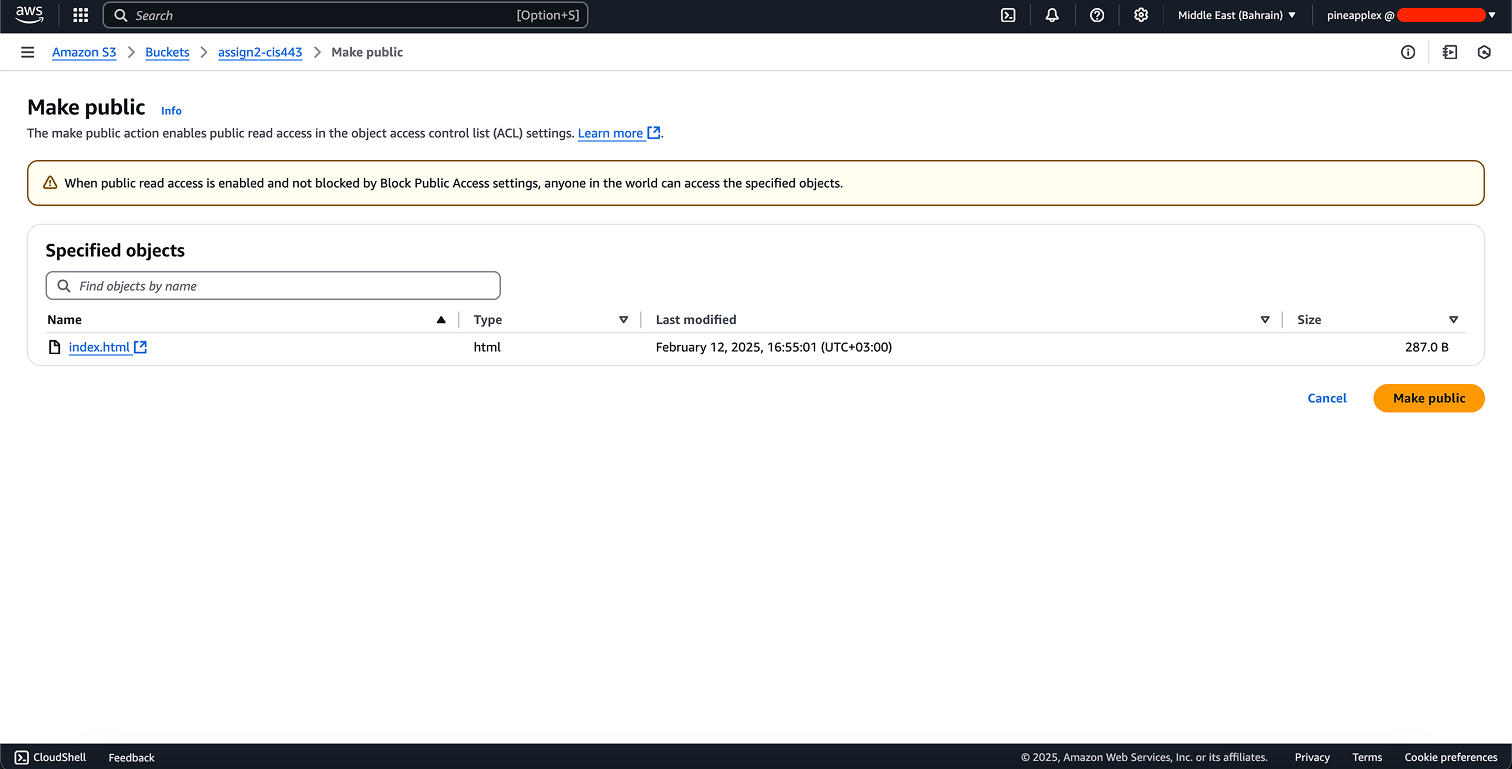
\includegraphics[width=0.95\textwidth]{host-static-website-12.png}
    \caption{S3 Static Website - Make Public Page}
    \label{fig:static12}
\end{figure}

\begin{figure}[H]
    \centering
    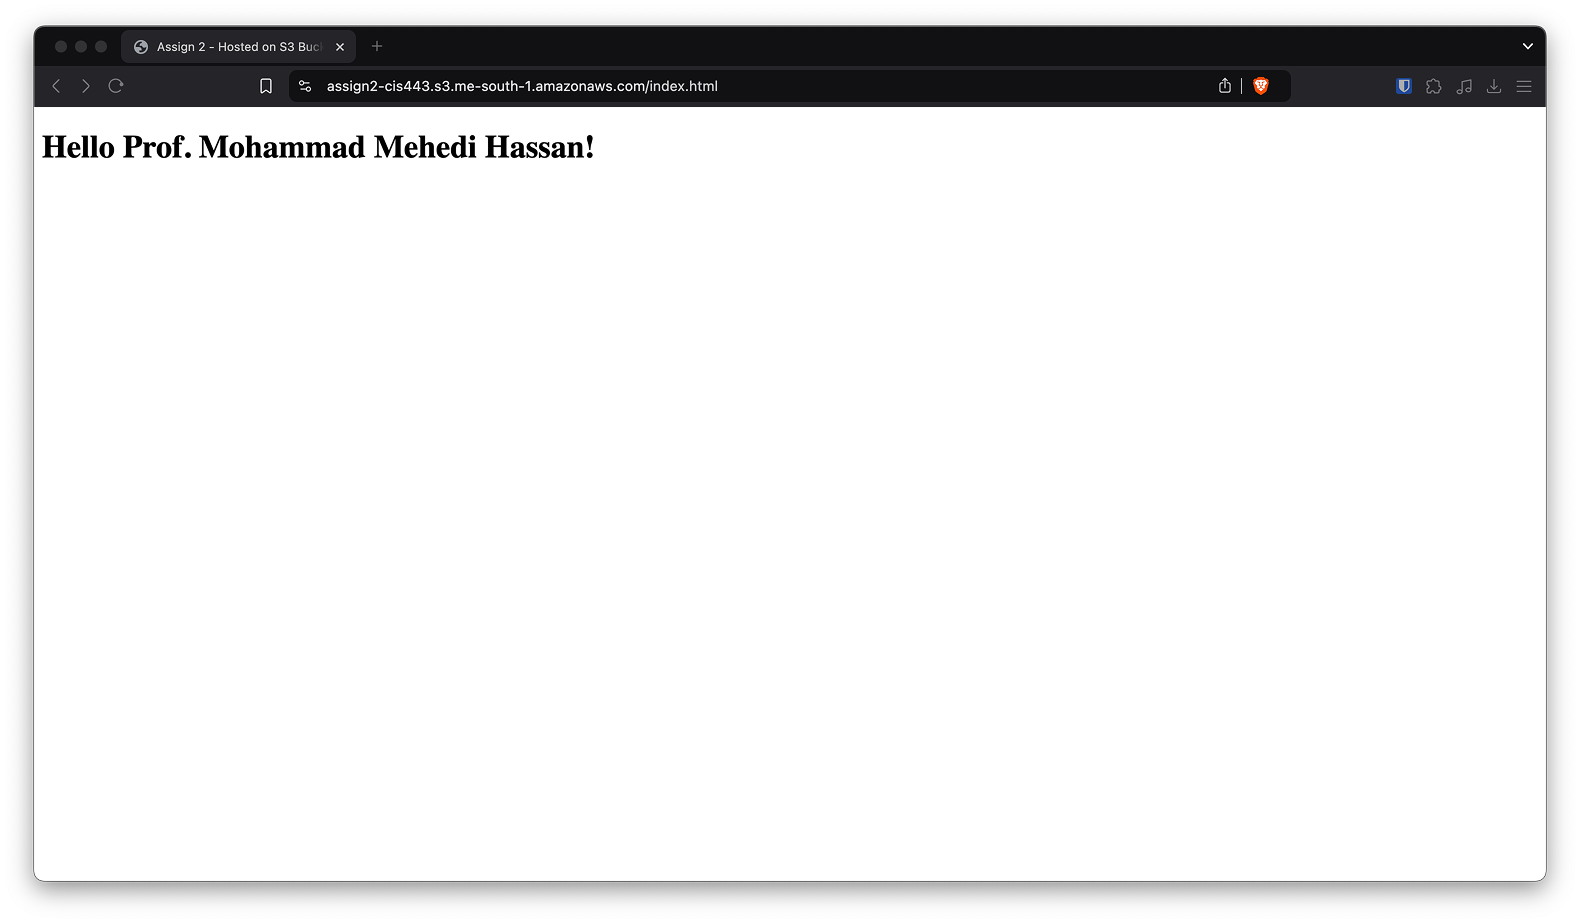
\includegraphics[width=0.95\textwidth]{host-static-website-13.png}
    \caption{Successfully hosted static website showing "Hello World"}
    \label{fig:static13}
\end{figure}

\end{document}
